\documentclass[a4paper,11pt]{scrreprt}

\usepackage[utf8]{inputenc}
\usepackage[ngerman]{babel}
\usepackage[T1]{fontenc}
\usepackage{amsmath}
\usepackage{graphicx}
\usepackage{xcolor}
\usepackage{wrapfig}
\usepackage{multirow}
\usepackage{ulem}
\usepackage{booktabs}
\usepackage{caption}
\usepackage{subcaption}
\usepackage{url}
\usepackage{fancyhdr}
\usepackage{lscape}
\usepackage{hyperref}
\usepackage{blindtext}
\usepackage{adjustbox}
\usepackage[top=3.5cm,bottom=3.5cm,left=2.5cm,right=2.5cm]{geometry}

\bibliographystyle{unsrt}
\parindent0pt

%Kopf-& Fusszeile----------------------------
\pagestyle{fancy}
\lhead{
\includegraphics[width=1.5cm]{Bilder/fhnw_logo.png}}
\chead{EIT}
\rhead{\slshape \leftmark}
\cfoot{\thepage}
\renewcommand{\headrulewidth}{0.4pt}
\renewcommand{\footrulewidth}{0.4pt}
%--------------------------------------------

\renewcommand*\chapterheadstartvskip{\vspace*{-0.2cm}}

\begin{document}
\thispagestyle{empty}

\begin{center}
\begin{tabular}{p{\textwidth}}

\begin{flushleft}

\includegraphics[scale=1.3]{Bilder/FHNW.png}
\end{flushleft}

\\

\\

\begin{center}
\textcolor{black}{
\textbf{
\Huge{
Fachbericht
}}}
\end{center}

\\

\begin{center}
\Large{
\textbf{
Projekt 4
}}
\end{center}

\\

\begin{center}
\large{
Fachhochschule Nordwestschweiz FHNW
}
\end{center}

\\

\begin{center}
\large{\today}
\end{center}

\vspace*{2cm}

\begin{center}
\begin{tabular}{ll}
\toprule 
\textbf{Studiengang:} 		& Elektro- und Informationstechnik EIT \\
\hline
\textbf{Auftraggeber/in:} 	& Prof. Hans Gysin\\
							& Jana Kalbermatter\\
\hline
\textbf{Fachexperten:} 		& Matthias Meier \\
							& Prof. Dr. Pascal Schleuniger \\
							& Pascal Buchschacher \\
							& Dr. Roswitha Dubach \\
							& Dr. Anita Gertiser \\
							& Bonnie Domenghino \\
\hline
\textbf{Projektteam:} & Adrian Annaheim \\ 
							& Benjamin Ebeling \\ 
 							& Jonas Rosenmund\\ 
 							& Michael Schwarz  \\ 
 							& Samuel Wey \\ 
 							& Andres Minder \\ 
\bottomrule
\end{tabular}
\end{center}

\end{tabular}
\end{center}
\newpage

\tableofcontents \thispagestyle{fancy}  \cfoot{} \renewcommand{\footrulewidth}{0pt} \rhead{\slshape Inhaltsverzeichnis}
\newpage

% ab hier ist diese Konvention für die Fusszeile eingestellt
\fancyfoot[C]{\thepage}
\fancyfoot[R]{\today}
\renewcommand{\footrulewidth}{0.4pt}

\chapter{Probe}
% ==================================================================
\setcounter{page}{1} \thispagestyle{fancy} 
\fancyhead[R]{chapter title}
% ==================================================================
\blindtext \cite{Minder2013}
\newpage

%\bibliography{Literaturverzeichnis/lit_pflichtenheft}
% ================ Einstellungen =======================
\thispagestyle{fancy} \addcontentsline{toc}{chapter}{Literaturverzeichnis} \rhead{\slshape Literaturverzeichnis}
% ======================================================

\newpage

\chapter{Anhang}
\label{Anhang}
% ================ Einstellungen =======================
\thispagestyle{fancy} \rhead{\slshape Anhang} 
% ============================================
\begin{figure}[h]
\centering
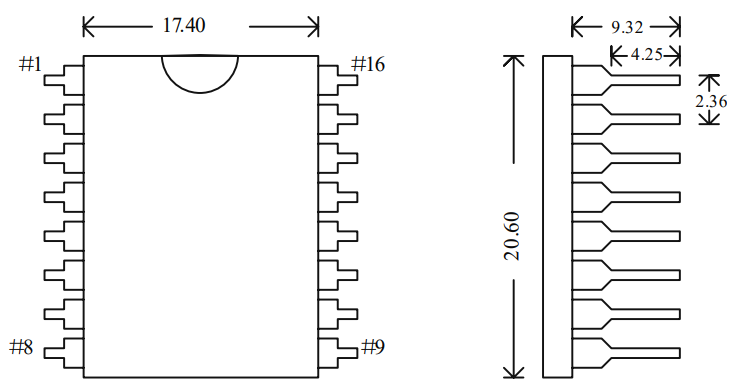
\includegraphics[scale=0.5]{Bilder/footprint_wtv020.png}
\label{fig:irgendesBild}
\caption[Abmessungen WTV020]{Abmessungen WTV020}
\end{figure}

\section{Benutzeranleitung}
\subsection{\texttt{maketicket inventory\_file preset\_file}}
Dieser CLI-Befehl schreibt ein "Ticket" auf das EEPROM.
Das inventory\_file beschreibt die ganze Datenbank, 
das preset\_file beschreibt, welche Audiodateien sich schon auf der SD-Karte befinden.
Gibt man den Befehl ein, promptet das Programm den Nutzer, 
welche Ausstellungen bezahlt sind und anschliessend welche Sprache gewünscht ist.
Sind diese Daten erfasst schreibt das Programm das Ticket über die serielle Schnittstelle auf das EEPROM.
\subsection{\texttt{makepackage inventory\_file preset\_file package\_path}}
Dieser CLI-Befehl kopiert die Audiodateien aller in der Presetdatei spezifizierter Ausstellungen in den Ordner package\_path. 
Die Dateien sind dann alle umbenannt, damit sie in der richtigen Reihenfolge auf die SD-Karte geschrieben werden.
\subsection{\texttt{loadsd package\_path}}
Dieser CLI-Befehl schreibt alle Audiodateien im Ordner package\_path auf die SD-Karte des Dojos. Alle schon auf der SD-Karte vorhandenen Dateien werden dabei gelöscht.

\newpage
Auf den folgenden Seiten befinden sich das Schema, das Layout und der Bestückungsplan der Printplatte.

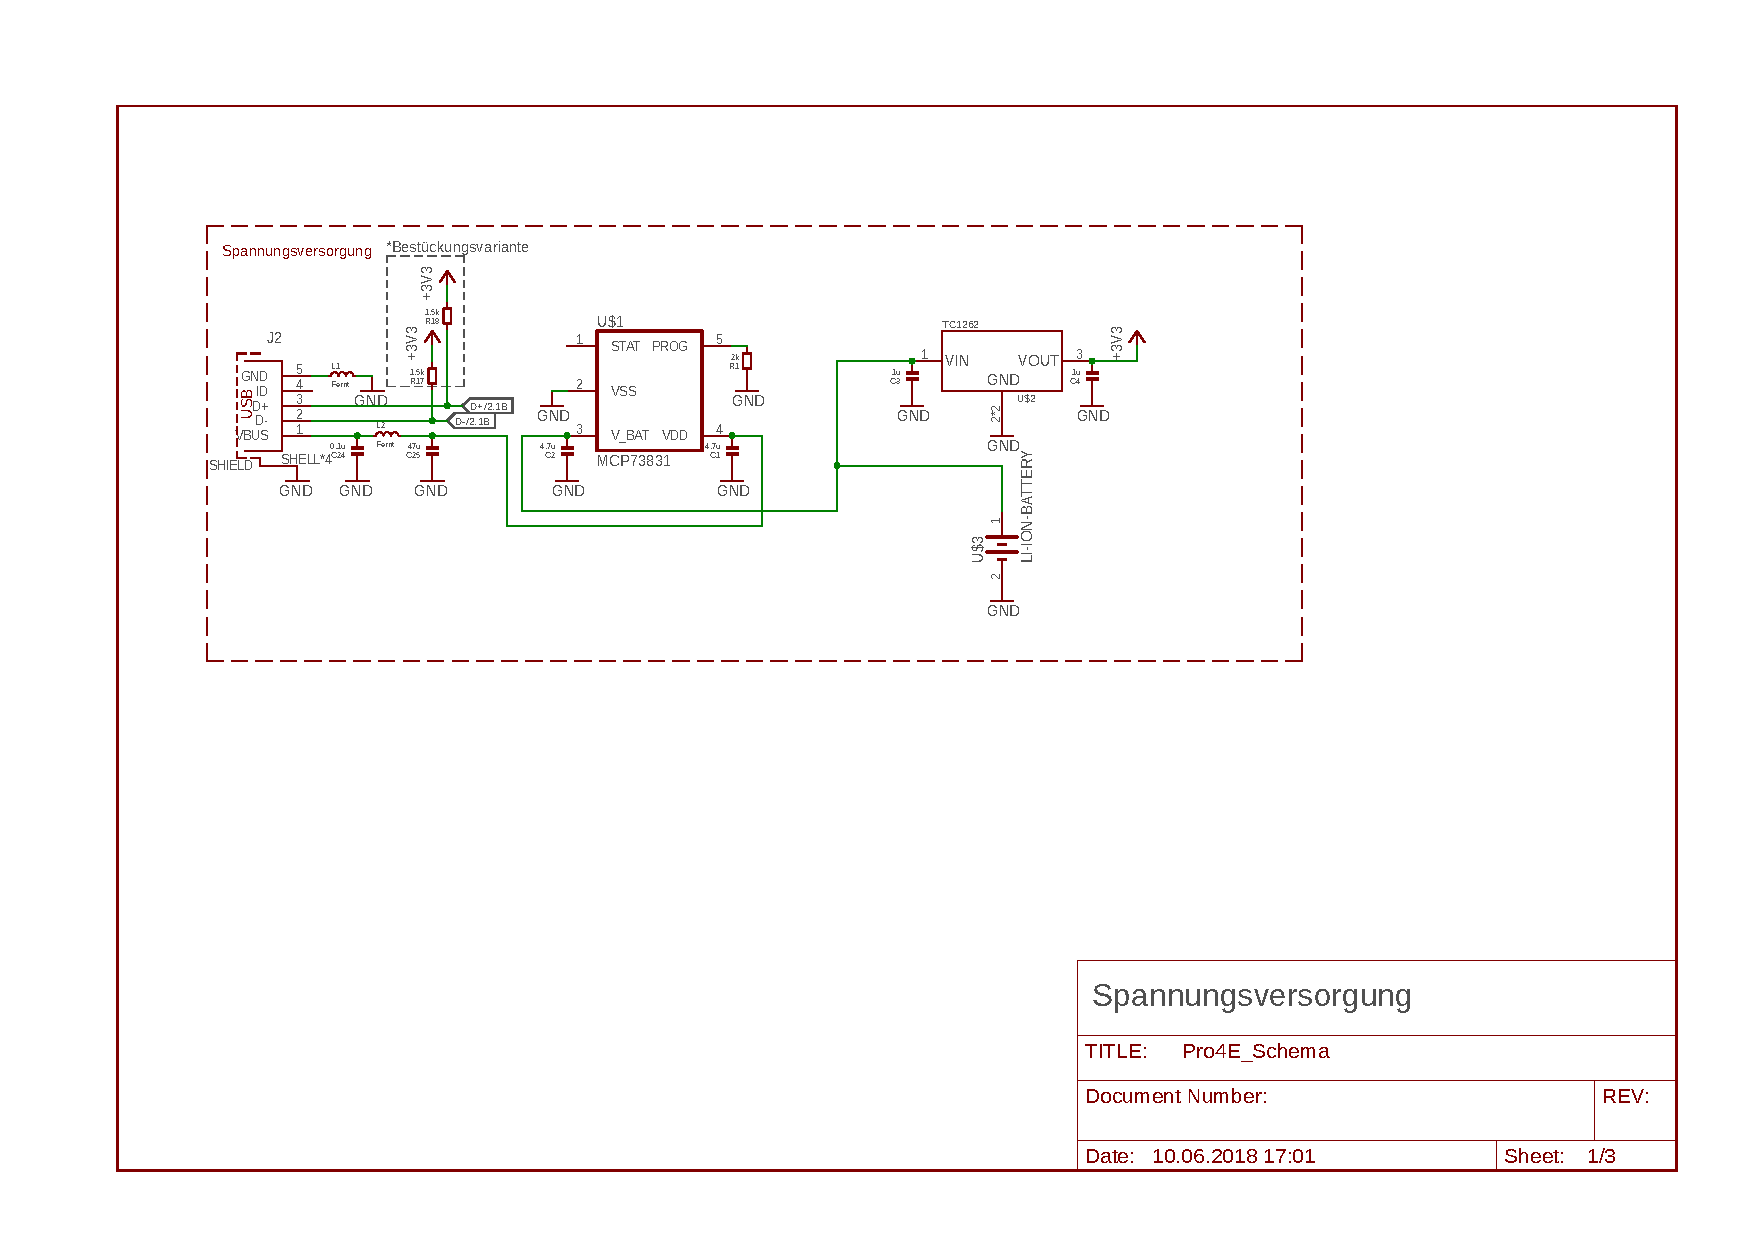
\includepdf[pages=1,fitpaper]{pdfs/Schema_Spannungsversorgung}
\label{pdf:SchemaSpannungsversorgung}

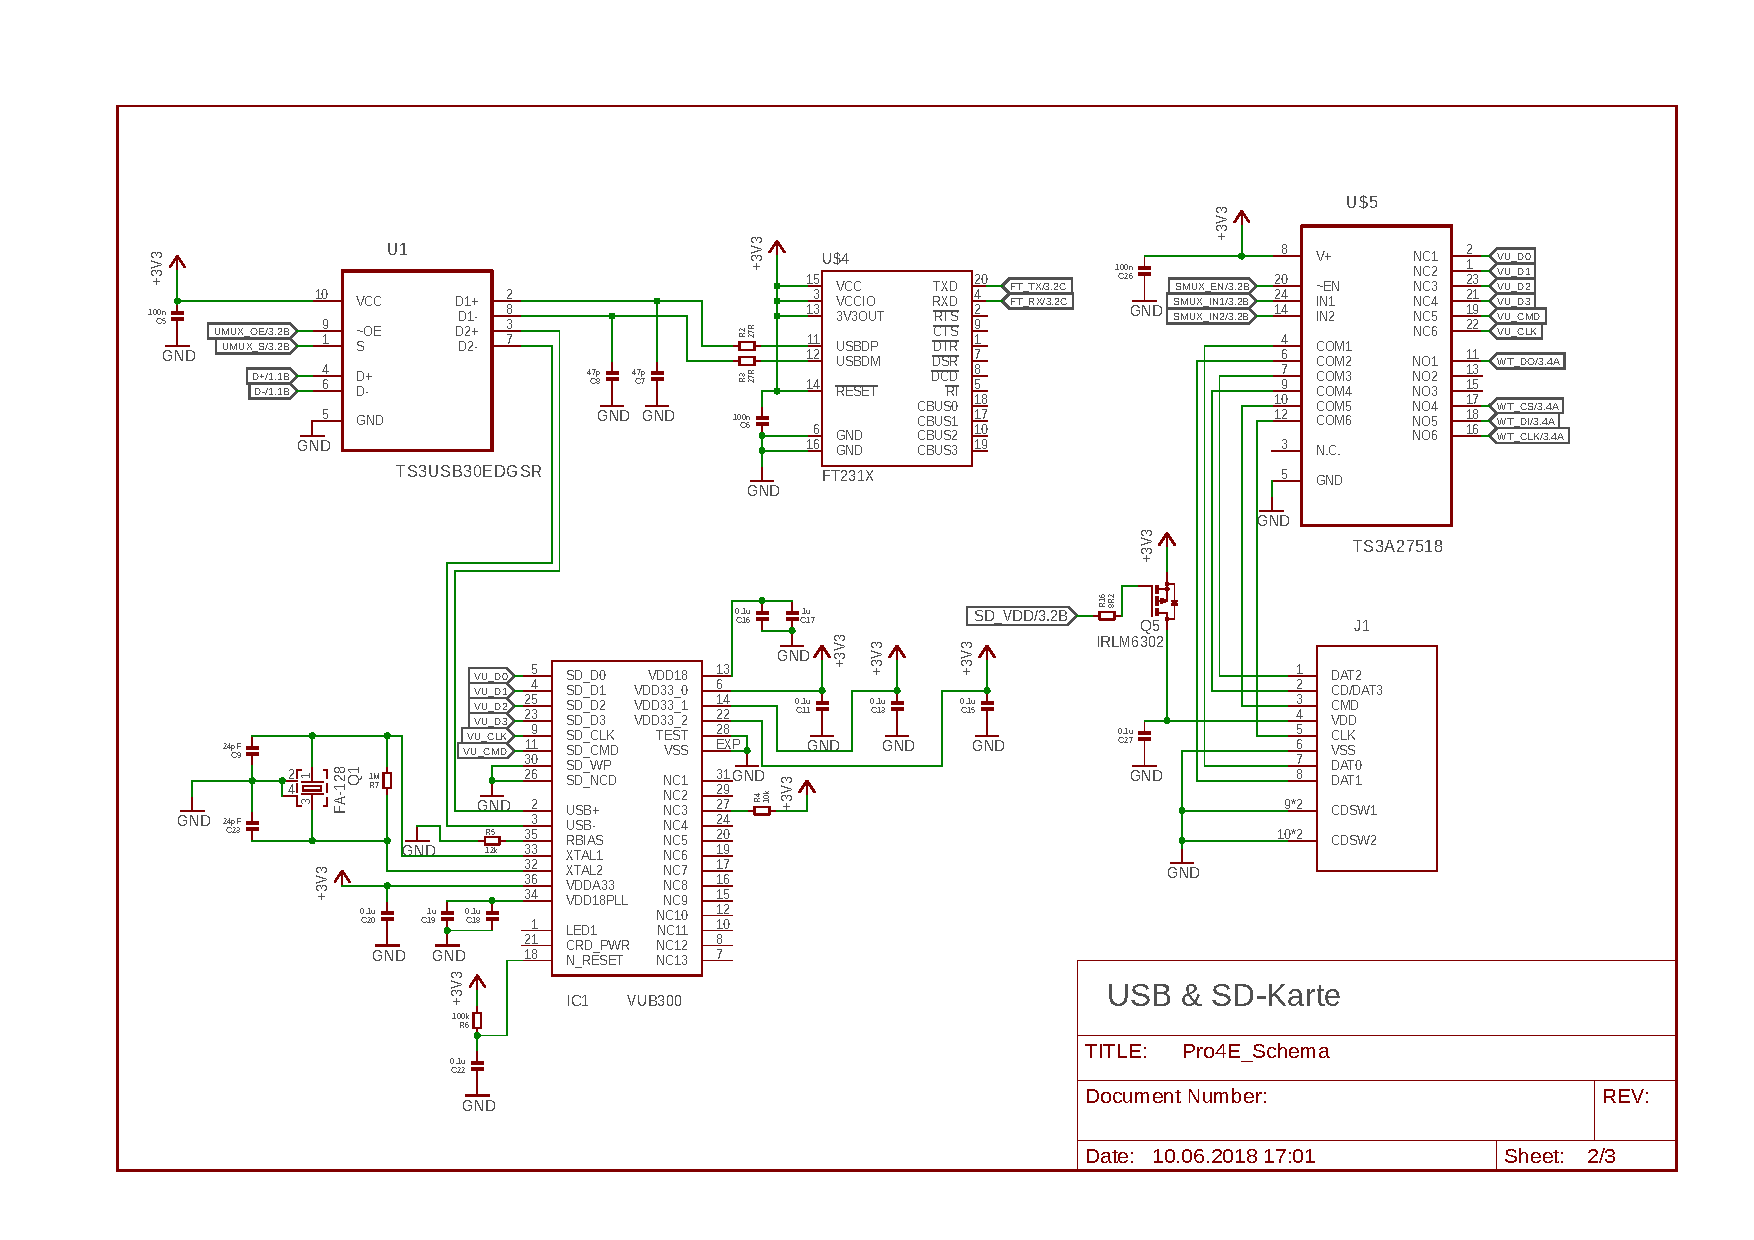
\includepdf[pages=1,fitpaper]{pdfs/Schema_USB}
\label{pdf:SchemaUSB}

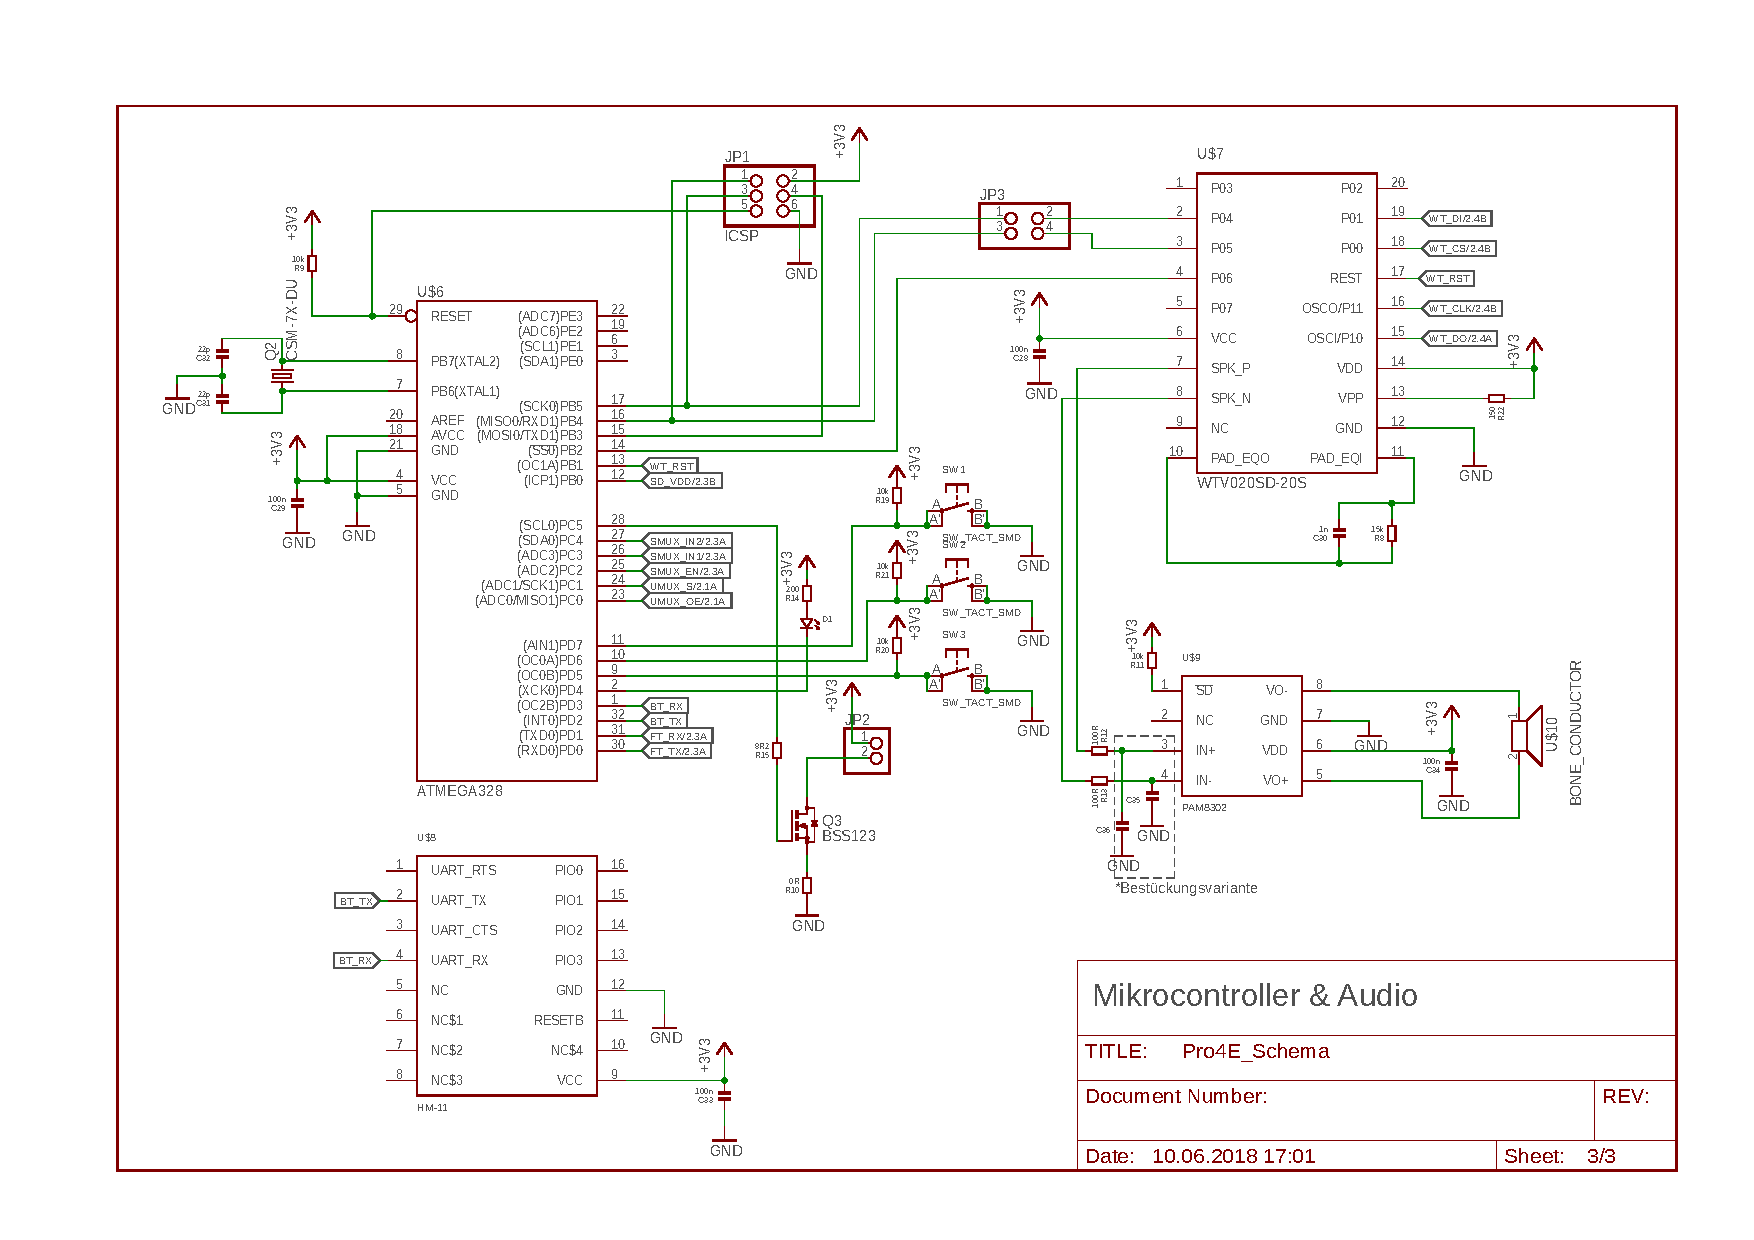
\includepdf[pages=1,fitpaper]{pdfs/Schema_Mikrocontroller}
\label{pdf:SchemaMikrocontroller}

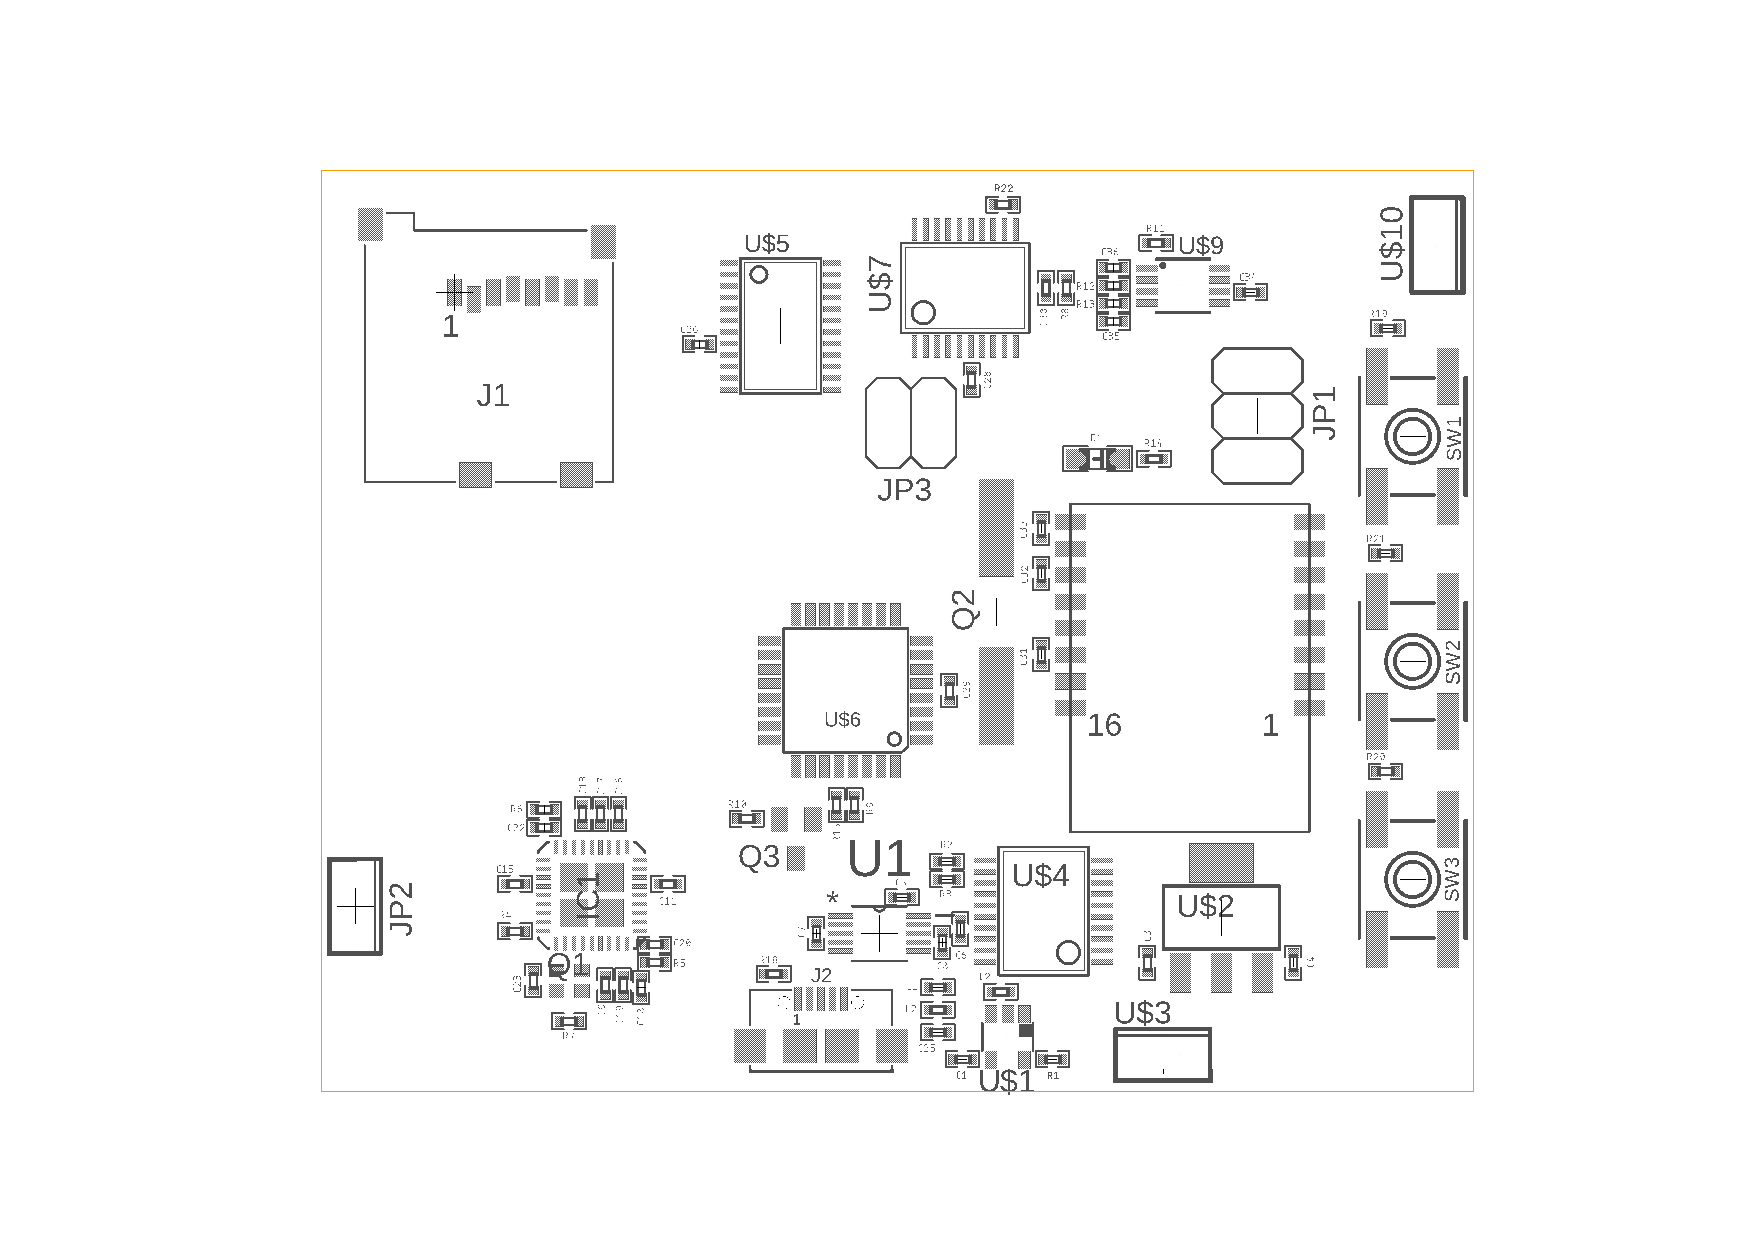
\includepdf[pages=1,fitpaper]{pdfs/Bestueckung_Top}
\label{pdf:BestueckungTop}

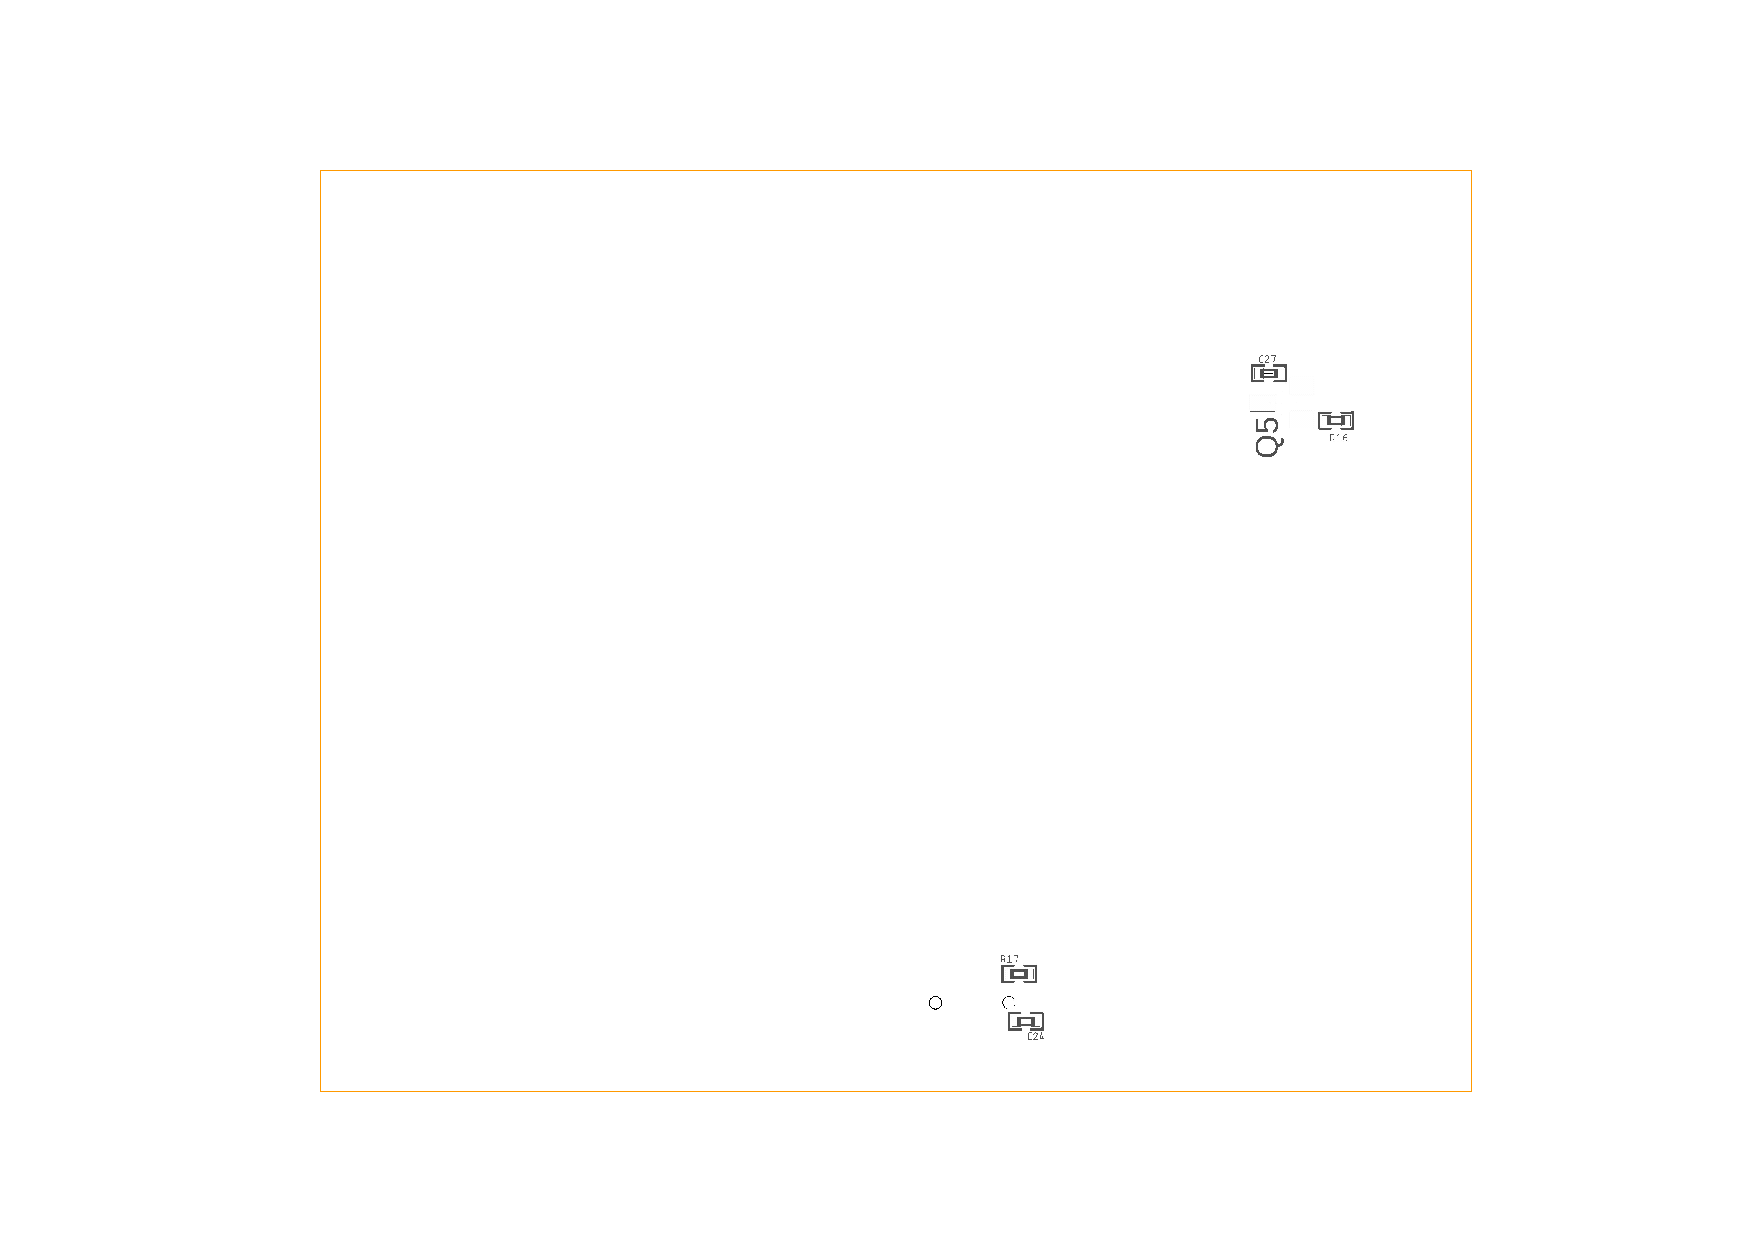
\includepdf[pages=1,fitpaper]{pdfs/Bestueckung_Bottom}
\label{pdf:BestueckungBottom}

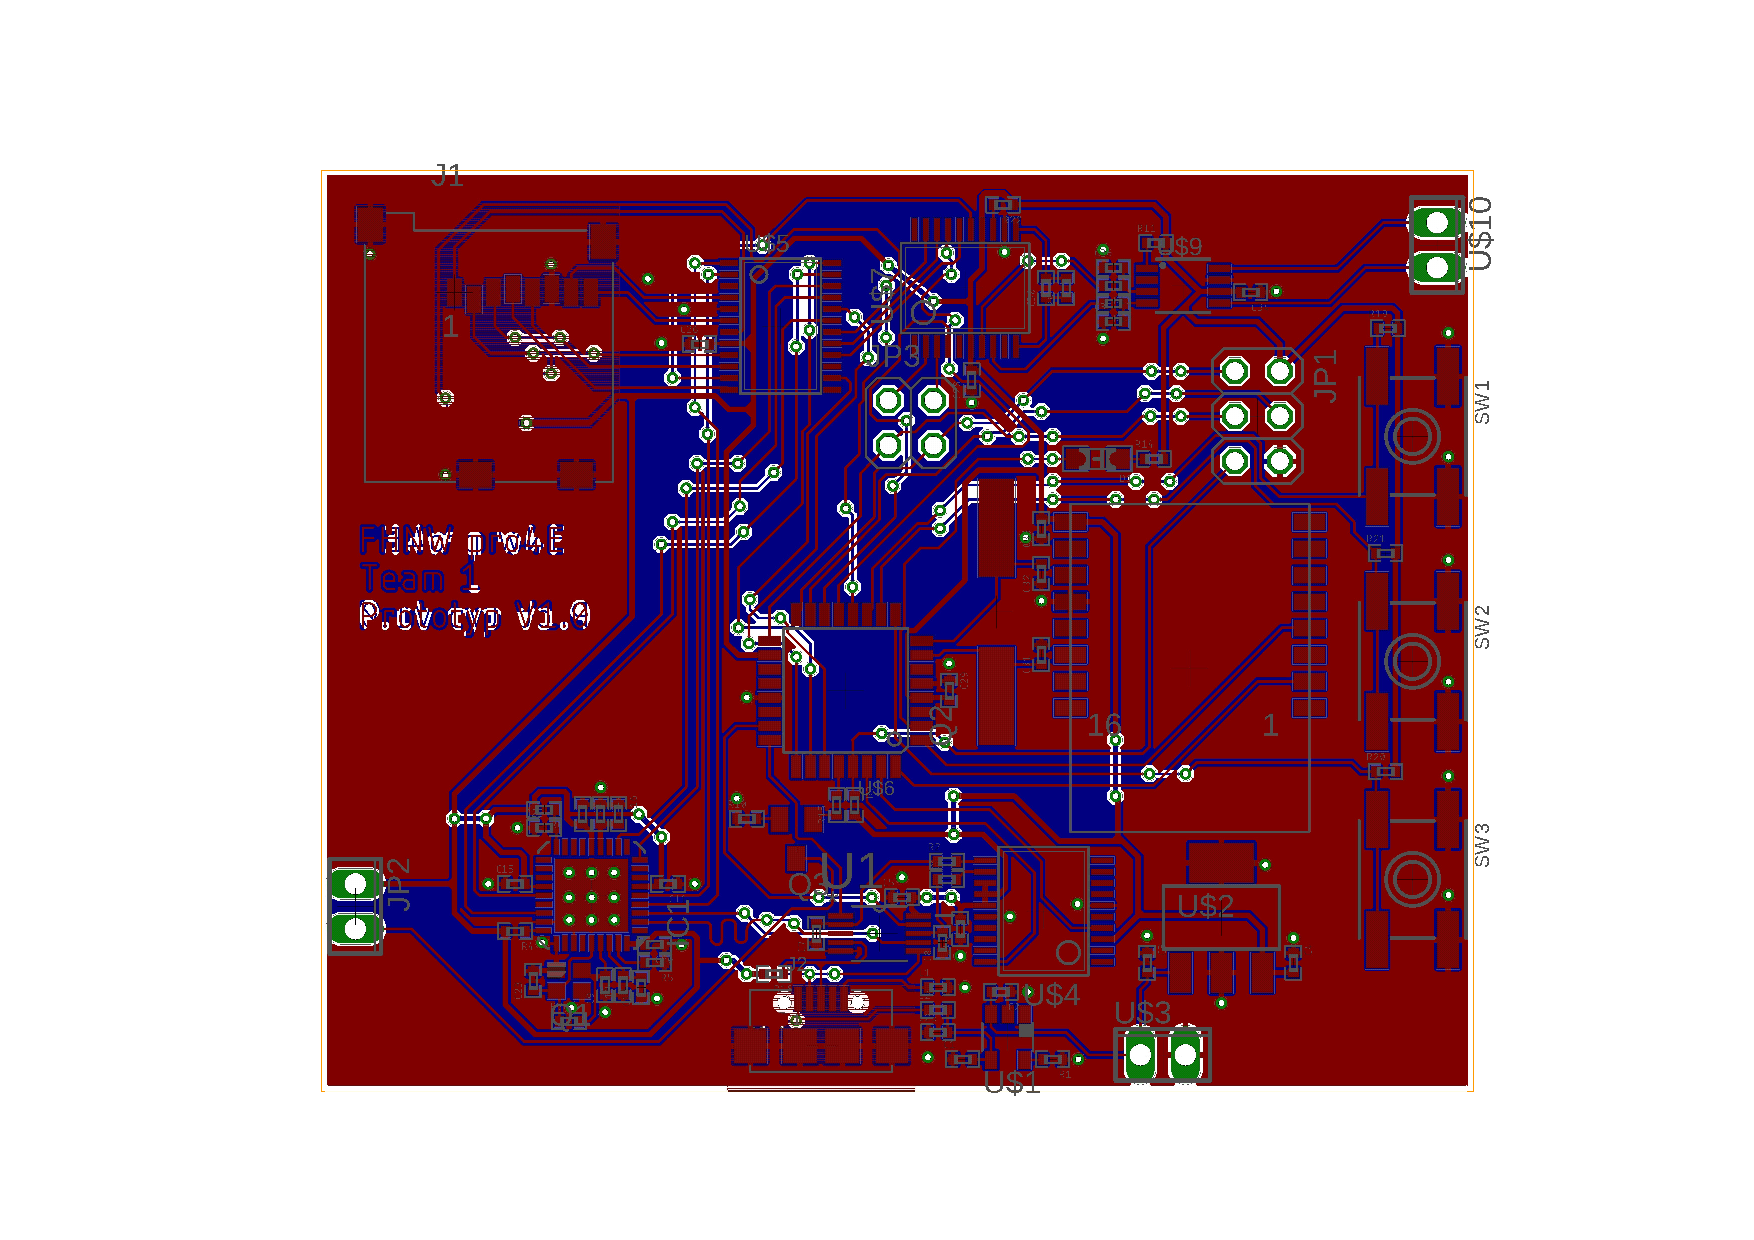
\includepdf[pages=1,fitpaper]{pdfs/Layout_all}
\label{pdf:LayoutAll}

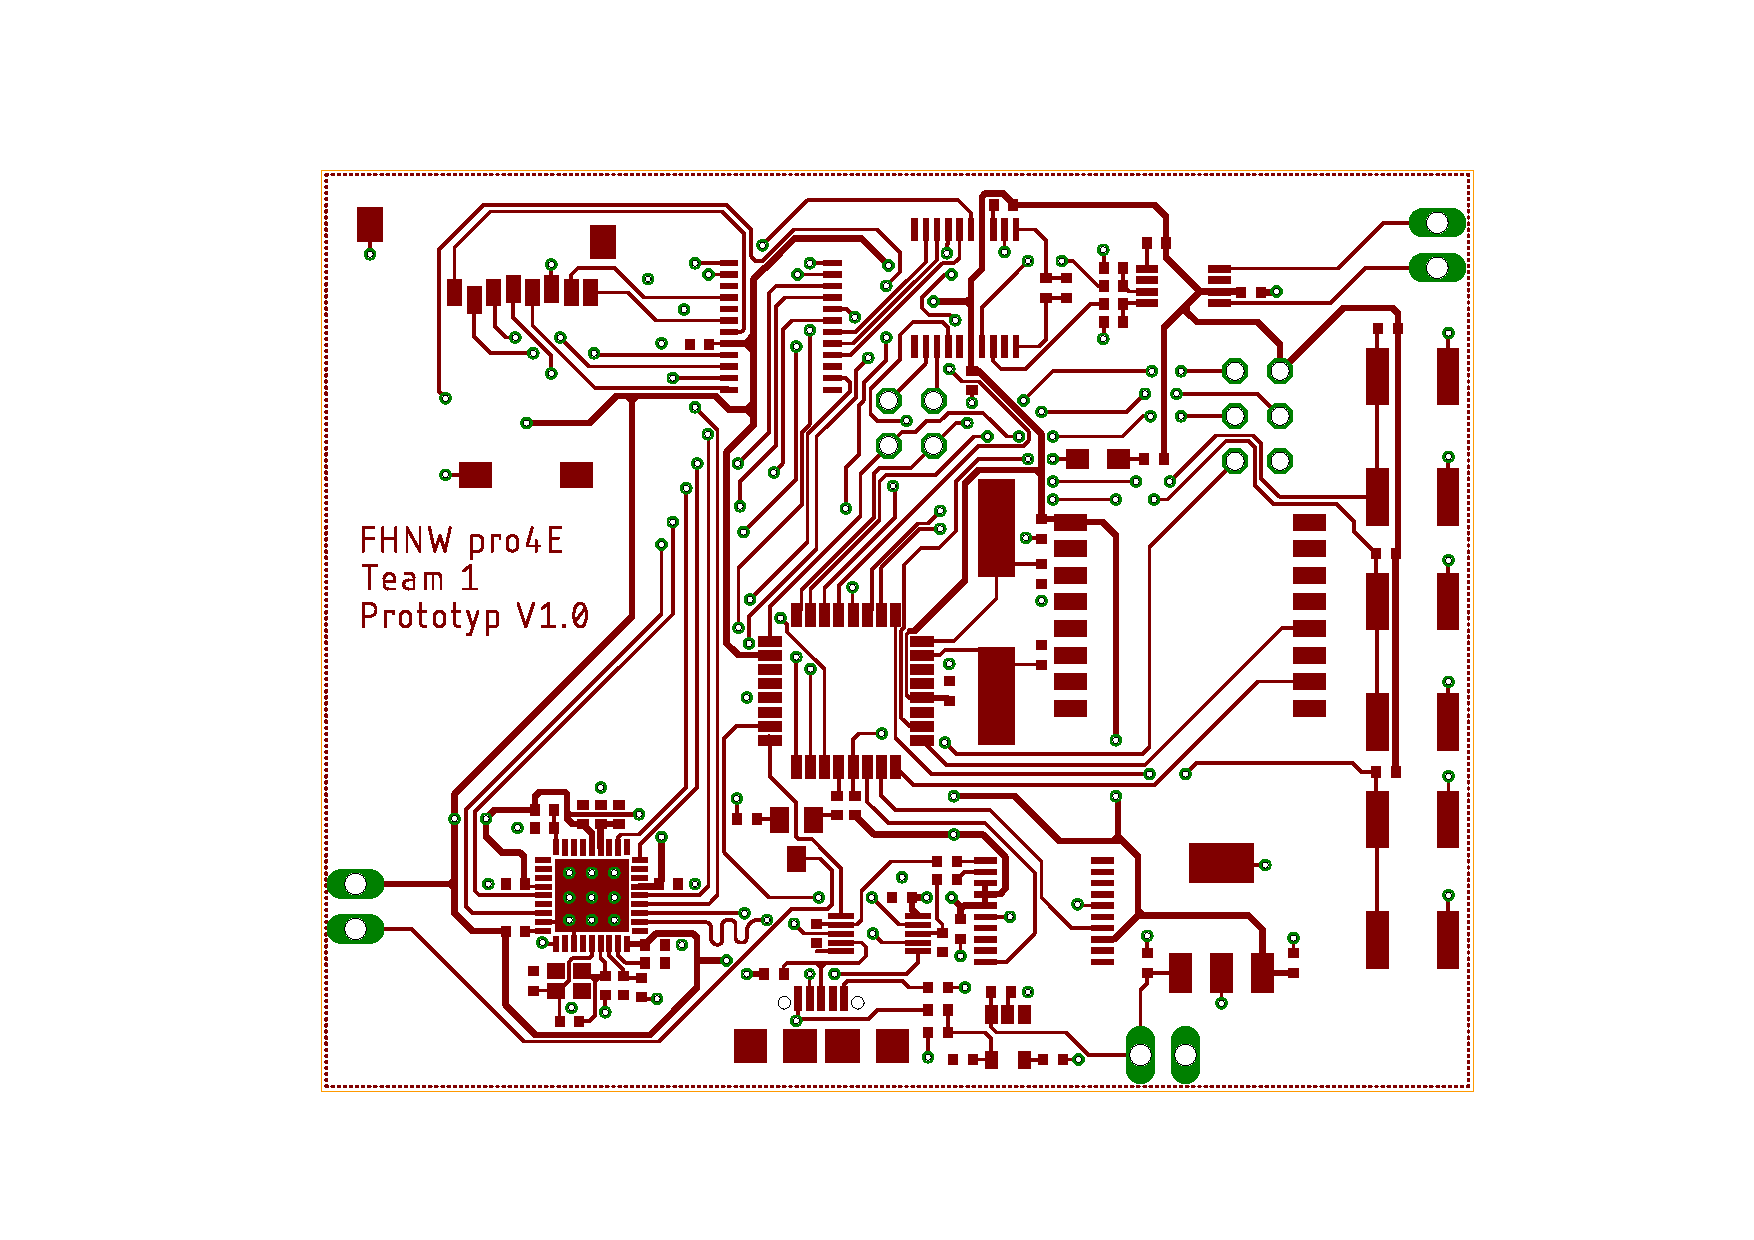
\includepdf[pages=1,fitpaper]{pdfs/Layout_top}
\label{pdf:LayoutTop}

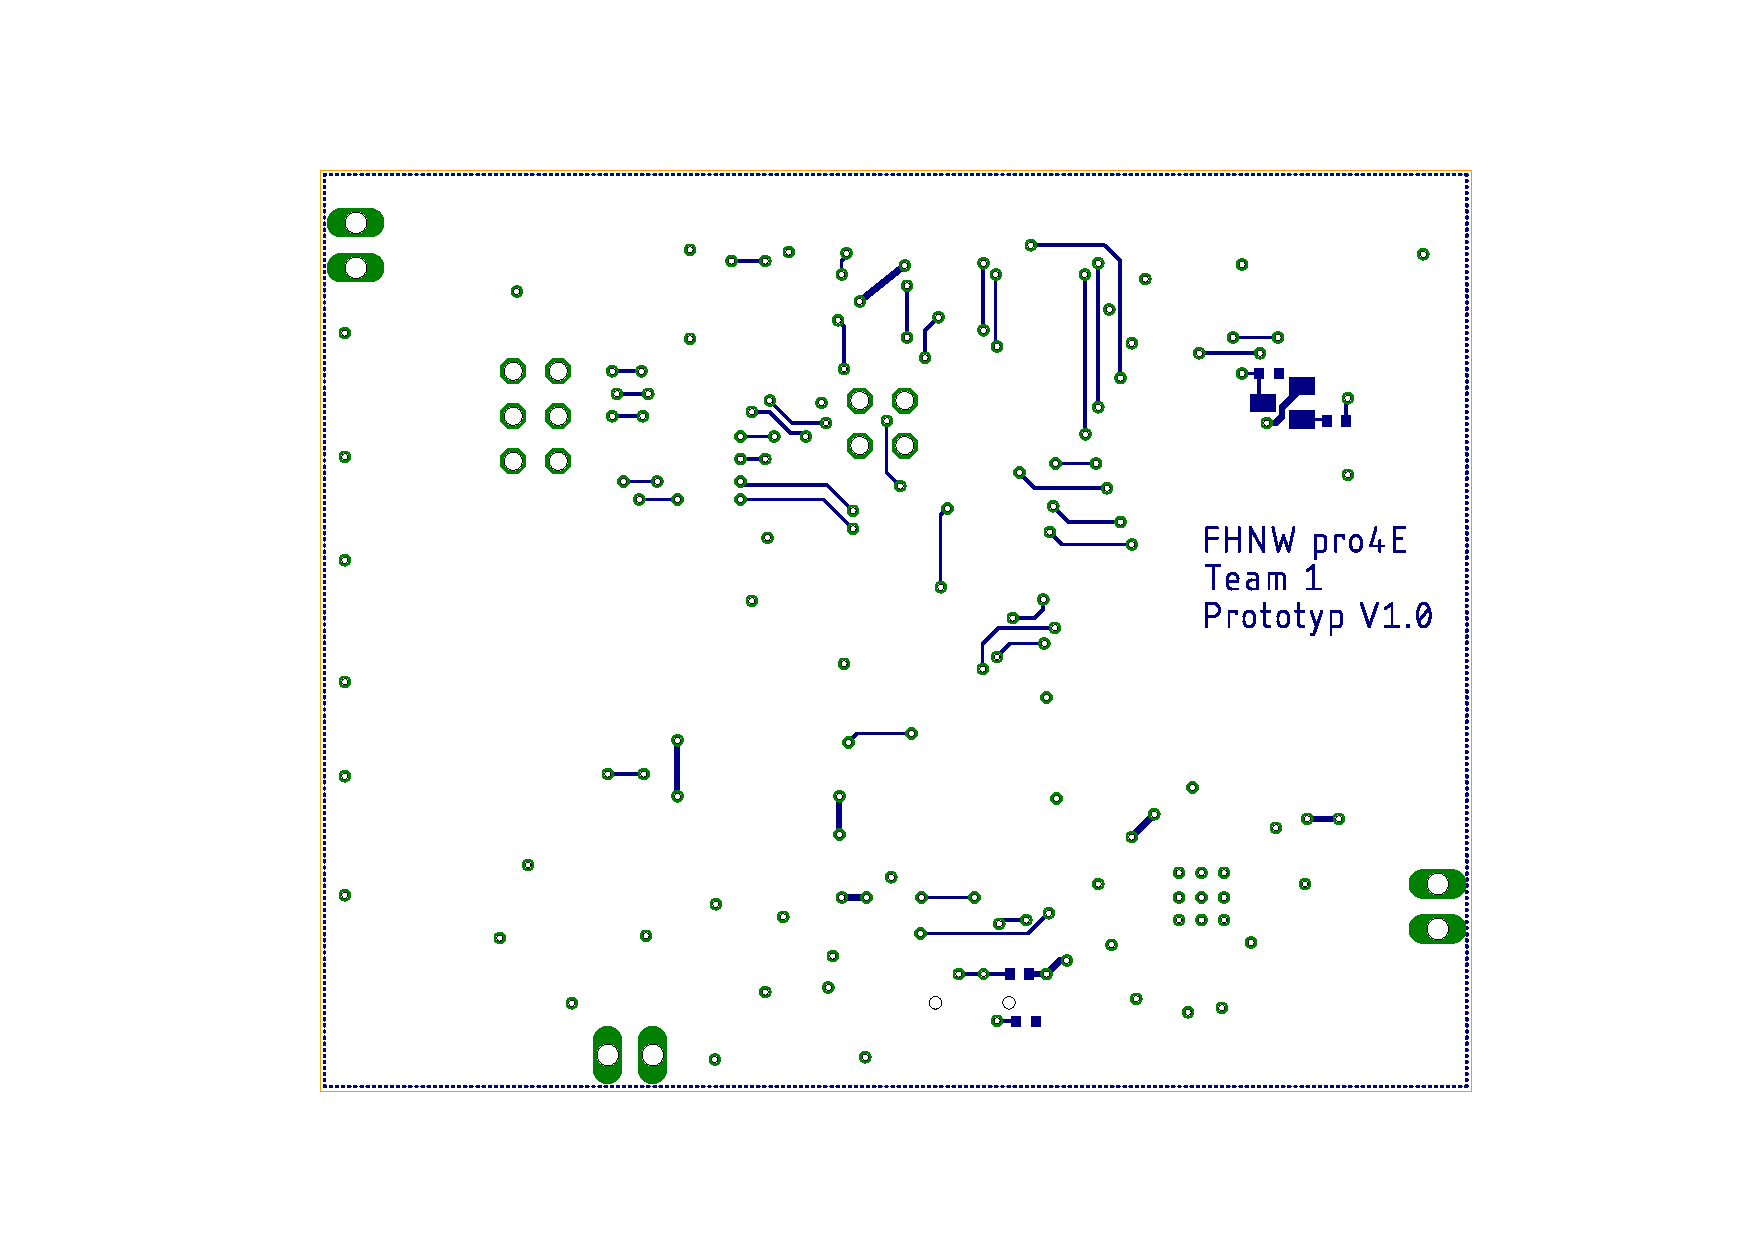
\includepdf[pages=1,fitpaper]{pdfs/Layout_bottom}
\label{pdf:LayoutBottom}

\newpage

\end{document}


